\chapter{Cluster Schedulers}

\section{Cluster Scheduling Principles}
	\subsubsection{Scheduling}
	Cluster \textbf{utilization }and \textbf{efficiency }are key indicators for good \textbf{resource management }and \textbf{scheduling decisions}. A better scheduling means smaller clusters as well as larger workloads with the same cluster size.
	\subsubsection{Multiplexing}
	The multiplexing of multiple, heterogeneous mixes of applications running concurrently complicates the scheduling problem.
	\subsubsection{Scalability}
	Cluster and workload size keep growing, and the scheduling complexity is roughly proportional to the cluster size. Schedulers must be scalable and bottlenecks have to be avoided.
	\subsubsection{Workload}
	The cluster scheduler must support heterogeneous workloads and clusters.\newline
	Clusters are made of several generations of machines and the workload evolves in time and is made of different applications. Generally there are two main job types: \textbf{batch jobs} (e.g. MapReduce computations) and \textbf{service jobs} (e.g. end-user facing a web service).\newline
	Knowing the workload of a cluster is fundamental, measurements can inform scheduling design, for example, about the differences between jobs in terms of number and runtime.

\section{Taxonomy of scheduling design issues}
	\textbf{Work Partitioning}\newline
	How to allocate work across frameworks: workload oblivious load balancing; partitioned workload and specialized schedulers; hybrid.\newline
	\newline
	\textbf{Resources choice}\newline
	Which clusters resources are made available to concurrent networks: all resources available; a subset is granted or offered\footnote{In this case the use of preemption primitives helps scheduling primitives but it can cause a waste of work.}.\newline
	\newline
	\textbf{Interference}\newline
	What to do when multiple frameworks attempt to use the same resources: make sure to avoid conflicts, partition resources across frameworks (\textbf{pessimistic concurrency control}) or, detect and undo conflicts if there are any (\textbf{optimistic concurrency control}).\newline
	\newline
	\textbf{Allocation granularity}\newline
	Task scheduling policies: atomic, all-or-nothing gang scheduling (e.g. Message Passing Interface programs); or incremental placement, hoarding (e.g. MapReduce).\newline
	\newline
	\textbf{Cluster-wide behaviour}\newline
	Requirements that need a global view like \textbf{fairness across frameworks} and \textbf{global notion of priority}.

\section{Schedulers Architectures}
	\subsubsection{Monolithic}
	Uses a \textbf{single centralized instance} that implements all the policies in a single code base. It applies the \textbf{same scheduling algorithm to all incoming jobs}.\newline
	A possible alternative is to add the support for multiple paths for different jobs, implementing different scheduling logic.\newline
	It is difficult to implement (add new scheduling policies) and to maintain (does not scale well to large clusters).
	\subsubsection{Statically partitioned}
	This is the standard approach: each framework has complete control over a set of resources (e.g. Hadoop 1.0), a single resource manager grants resources to independent \textit{framework schedulers}.\newline
	It can schedule between \textbf{multiple frameworks} but it has to deal with the problems of static partitioning: \textbf{fragmentation of resources} and \textbf{sub-optimal utilization} of the cluster.
	\begin{figure}[H]
		\centering
		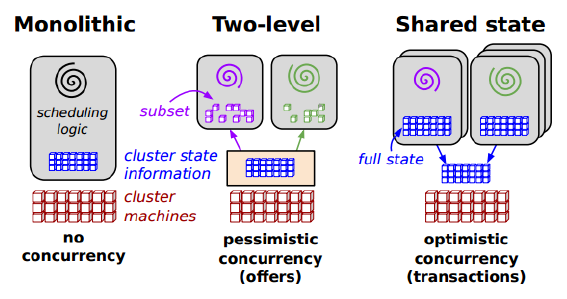
\includegraphics[width=0.5\linewidth]{images/clust_sched_arch.png}
		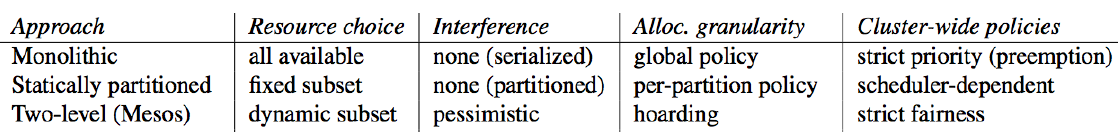
\includegraphics[width=\linewidth]{images/clust_sched_comparison.png}
		\caption{\textit{Comparison of cluster scheduling approaches.}}
	\end{figure}
	\subsubsection{Two-levels}
	It uses a \textbf{coordinator} to \textbf{dynamically allocate resources} to concurrent frameworks.\newline
	An example is \textbf{Mesos}, it makes exclusive resource offers to the frameworks, they lock resources by acccepting the offers (pessimistic concurrency control). No global cluster state is available to frameworks.\newline
	The \textbf{YARN} scheduler is closer to a monolithic architecture. It has a centralized resource allocator (RM) with per-job framework master (AM), but the latter only provides job management services (no scheduling).
	\subsubsection{Shared-state}
	Multiple replicas of cluster state are independently updated by application-level schedulers. After the change is applied locally, the scheduler issues an optimistically concurrent transaction to update the shared cluster state (e.g. Google's Omega).

\section{YARN}
	\subsection{Previous limitations and improvements}
		\subsubsection{Hadoop 0.1 limitations}
		It \textbf{only supports MapReduce} and it has \textbf{scalability issues}. System failures destroy running and queued jobs (\textbf{poor availability}). \textbf{Sub-optimal resource utilization}: static partitioning of resources in Map or Reduce slots.
		\subsubsection{YARN improvements}
		\textbf{Support for multiple applications}. Separate resource management from application logic and share same Hadoop cluster across applications.\newline
		\newline
		\textbf{Improved cluster utilization}. Generic resource \textit{container} model replaces fixed Map/Reduce slots. Container allocation based on locality and memory.\newline
		\newline
		\textbf{Improved scalability}. Remove complex application logic from the resource manager. Compact scheduling protocol. Message passing based on loosely coupled design.\newline
		\newline
		\textbf{Application agility}. Use protocol buffers for RPC (Remote Procedure Call) gives wire compatibility. MapReduce becomes an application in user space. Multiple versions of an application can co-exist. Easier upgrade of framework and applications.\newline
		\newline
		\textbf{Shared services}. Common services in a pluggable framework. Distributed file sharing service. Remote data read service. Log aggregation service.
		 
	\subsection{Architecture and Core Components}
	Nodes resources are allocated to applications on request (\textbf{dynamic resource partitioning}), there are no more slots.\newline
	Separate resource management from application logic: cluster-wide resource allocation and management with per-application master component.
		\subsubsection{Schedulers}
		Schedulers are pluggable components of the RM, in addition to the existing ones, advanced scheduling is supported. Currently supported schedulers are the capacity scheduler and the fair scheduler, it also supports Dominant Resource Fairness and Hierarchical Queues.
		\subsubsection{Resource Manager [RM]}
		The RM runs on the master node and arbitrates system resources between competing applications.\newline
		It tracks heartbeats from Node Managers (\textbf{Node management}).\newline
		It handles to the Application Master the requests for new containers and de-allocates them when they expire or the application finishes (\textbf{containers management}).\newline
		It creates a container for each new AM and tracks its health (\textbf{AM management}).\newline
		It integrate Kerberos (\textbf{Security management}).
		\subsubsection{Node Manager [NM]}
		The Node Manager runs on slave nodes, it \textbf{handles communications with the RM}: it registers, monitors and communicates node resources, and sends heartbeats and container status.\newline
		It \textbf{manages processes in containers}: launches AMs on request from the RM and launches applications on request from the AMs. Furthermore, it \textbf{monitors resource usage and kills processes and containers}.\newline
		Finally, it p\textbf{rovides log services}: Log Aggregation and roll over to HDFS.\newline
		The shuffle mechanism is an auxiliary service that runs un the NM JVM as a persistent service.
		\subsubsection{Resource containers}
		They are created by the RM upon request. They allocate a certain amount of resources on slave nodes for the applications to run.\newline
		The container launch context contains a container ID, the commands to start the application task, the environment configuration and local resources (application binary, HDFS files).
		\subsubsection{Application master [AM]}
		It is application specific, it runs in a container and requests one or more containers to execute application tasks.\newline
		A \textbf{resource request} contains a resource name (hostname, rackname, *), a priority (within the same application), resource requirements (memory, CPU) and the number of containers needed.
	\subsection{Fault tolerance}
		\subsubsection{Container failure}
		The AM reattempts containers that complete with exceptions or fails. Applications with too many failed containers are considered failed.
		\subsubsection{AM failure}
		If the application or the AM fails, the RM will re-attempt the whole application. Optionally the \textit{job recovery} could be set, it uses state to find which containers succeeded and which failed, and reschedules only the latter.
		\subsubsection{NM failure}
		If NM stops sending heartbeats; the RM removes it from the active nodes list and reschedules the containers on the filed node. AMs on the failed node are resubmitted completely.
		\subsubsection{RM failure}
		No application can be run if the RM is down. It can work in active/passive mode (like the Name Node of HDFS).
	
\section{MESOS}
	\subsection{Introduction and Motivations}
	Clusters of commodity servers are a major
	computing platform. To simplify the programming of the cluster, a diverse array of	cluster computing frameworks have been developed, but no framework will be optimal for all applications. Therefore, it is necessary to run multiple frameworks in the same cluster.\newline Multiplexing a cluster between frameworks improves utilization and	allows applications to share access to large datasets that	may be too costly to replicate across clusters. Two solutions for sharing a cluster are either to statically partition the cluster or to allocate a set of VMs to each
	framework. Unfortunately, these solutions achieve neither
	high utilization nor efficient data sharing. The main
	problem is the mismatch between the allocation granularities
	of these solutions and of existing frameworks.\newline
	\newline
	The short duration of tasks and the ability to run multiple tasks per node allow jobs to achieve high data locality, as each job will quickly get a chance to run on nodes storing its input data. Short	tasks also allow frameworks to achieve high utilization,	as jobs can rapidly scale when new nodes become available.
	Unfortunately, because these frameworks are developed
	independently, there is no way to perform fine grained
	sharing across frameworks, making it difficult to
	share clusters and data efficiently between them.\newline
	\newline
	A centralized approach would need to take as input framework requirements, resource availability, and organizational policies,
	and compute a global schedule for all tasks. This approach has to face several challenges.\newline
	The scheduler would need to provide a sufficiently expressive
	API to capture all frameworks’ requirements, and
	to solve an online optimization problem for millions
	of tasks. Even if such a scheduler were feasible, this
	complexity would have a negative impact on its scalability
	and resilience. Moreover, many existing
	frameworks implement their own sophisticated scheduling, and moving this functionality to a global
	scheduler would require expensive refactoring.\newline
	\newline
	Mesos uses a decentralized approach: it delegates
	control over scheduling to the frameworks. This is accomplished through the abstraction of \textit{resource
	offer}.\newline
	Mesos decides how many resources to offer each framework,
	while frameworks decide which resources to accept
	and which tasks to run on them. This decentralized
	scheduling model allows frameworks to meet
	goals such as data locality nearly perfectly. In addition,
	resource offers are simple and efficient to implement, allowing Mesos to be highly scalable and robust to failures.\newline
	\newline
	The typical workloads in data warehouse systems using Mesos includes: heterogeneous MapReduce jobs, production and had-hoc queries; large scale machine learning; SQL-like queries.
	\subsection{Architecture}
	The design philosophy is to have a scalable and resilient core exposing low level interfaces and to use high level libraries for common functionalities.\newline
	Mesos manages cluster resources while the frameworks control task scheduling and execution.\newline
	The two levels approach lets frameworks be independent so that they can support diverse scheduling requirements.
		\subsubsection{Mesos Master}
		It implements the first level scheduling. It uses resource offers (lists of free resources on multiple slaves) to implement fine-grained sharing. It collects resource utilization from slaves and implements cluster-wide allocation policy (Fair Sharing or Priority based).\newline
		Mesos also implements filters to optimize the resource offers mechanism (filter based on machine or resources). Frameworks can decide to reject an offer and wait for offers satisfying application constraints.\newline
		The master incentives the frameworks to speed up the offers mechanism by counting offers to a framework, it can also decide to invalidate an offer to avoid blocking or misbehaviours.
		\subsubsection{Mesos Frameworks}
		Each framework decides how to execute a job and its tasks\footnote{The actual task execution is requested by the master.}. Each framework has one scheduler and one executor per application. The framework scheduler registers to the master, selects which offer to accept and describes the tasks to launch on accepted resources.\newline
		The framework executor is launched on Mesos slaves executing on accepted resources, it takes care of running the framework's tasks.
		\subsubsection{Resource allocation and revocation}
		Resource allocation is done through a pluggable allocation module which can use either max-min fairness or strict priority.\newline
		It works under the assumption that tasks are short because Mesos only reallocates resource when tasks finish.\newline
		Unfortunately some jobs (e.g. streaming) may have long tasks, in this case Mesos can kill running tasks. Some applications (e.g. MPI) may be harmed by this mechanism more than others (e.g. MapReduce), therefore Mesos implements a guaranteed allocation mechanism: a minimum set of resources granted to a framework, if a framework is below his guaranteed allocation then Mesos never kills tasks, otherwise it could kill any of them.
		\subsubsection{Performance Isolation}
		Isolation between executors on the same slave is achieved through low-level OS primitives (pluggable isolation module). The currently supported mechanisms can limit CPU, memory, network and I/O bandwidth using Linux Containers and Solaris Cages.\newline
		This approach offers better isolation than the previous process-based approach but fine grained isolation is not yet fully functional.
		\subsubsection{Fault Tolerance}
		The master is designed with a soft state containing the list of active slaves, the list of registered frameworks and the list of running tasks.\newline
		Multiple masters stay in a hot-standby mode handled by zookeeper, upon failure a new master is elected (\textit{leader election}), slaves and executors help populate the new master's state.\newline
		In order to help frameworks tolerate failures, the master send health reports to the schedulers and allows multiple schedulers for a single framework.
	\subsection{Behaviour}
	The ideal Mesos workload has elastic frameworks, supporting scaling up and down seamlessly. Tasks duration has to me homogeneous and short and there has to be no strict preference over cluster nodes.\newline
	In the case a framework has cluster node preferences, Mesos can emulate a centralized scheduler offering cluster and framework wide resource sharing.
		\subsubsection{Definitions and metrics}
		\textbf{Elasticity} describes the capacity of a workload to use resources as soon as they are acquired and release them as soon as tasks finish.\newline
		\textbf{Task runtime distribution} measures homogeneity/heterogeneity of a workload.\newline
		\textbf{Mandatory resource} are required by a framework to work (assumption: mandatory resources < guaranteed share).\newline
		\textbf{Preferred resources} are resources that a framework should acquire to achieve better performance but are not fundamental for the job to work.\newline
		\newline
		\textbf{Framework ramp-up time} is the time it takes a new framework to get its fair share.\newline
		\textbf{Job completion time} is the time it takes a job to complete (assuming one job per framework).\newline
		\textbf{System utilization} is the total cluster resources utilization, with focus on CPU and memory.
		\subsubsection{Homogeneous and heterogeneous tasks}
		When dealing with a homogeneous workload there exist two cases: if there is a configuration satisfying all frameworks constraints the system will eventually converge to this optimal allocation; if no such allocation exists (e.g. demand is larger than supply) then lottery scheduling is used to achieve a weighted fair allocation.\newline
		If Mesos is dealing with an heterogeneous workload, then the worst case scenario happens when all nodes required by a short job are filled with long tasks. Fortunately the probability of such an event is small.
		\subsubsection{Limitations of Distributed Scheduling}
		\textbf{Fragmentation}: distributed collection of frameworks might not achieve the same packing quality of a centralized scheduler, this is mitigated by the use of big nodes (many CPUs, many cores) running small tasks.\newline
		\textbf{Starvation}: Large jobs may wait indefinitely for slots to become free because they are monopolized by small tasks from small jobs. This is mitigated by a \textit{minimum offer size} mechanism.
		
\section{BORG}
	\subsection{Introduction}
	Borg provides three main benefits: it \textbf{hides the details
	of resource management and failure handling} so its users can
	focus on application development instead; \textbf{operates with very high reliability and availability}, and supports applications that do the same; and lets us \textbf{run workloads across
	tens of thousands of machines effectively}.
	
	\subsection{User Perspective}
	Users submit their work to Borg	in the form of \textit{jobs}, each of which consists of one or more
	\textit{tasks} that all run the same program (binary). Each job runs in one Borg \textit{cell}, a set of machines that are managed as a
	unit.
		\subsubsection{Workloads}
		Borg cells run a heterogenous workload with two main parts.\newline
		The first is \textbf{long-running services} (mostly production, high-priority) that should “never” go down, and handle short-lived latency-sensitive requests (end-user-facing products such as Gmail or Google Docs).\newline
		The second is \textbf{batch jobs} that take from a few seconds to a few days to complete; these are much less sensitive to short-term performance fluctuations.\newline
		\newline
		The workload mix varies across cells, which run different mixes of applications depending on their major tenants (e.g., some cells are quite batch-intensive), and also varies over time: batch jobs come and go, and many end-user-facing service jobs see a	diurnal usage pattern. 
		\subsubsection{Clusters and cells}
		The machines in a cell belong to a single cluster, defined by the high-performance datacenter-scale network fabric that connects them.\newline
		A cluster lives inside a single datacenter building, and a collection of buildings makes up a site. A cluster usually hosts one large cell and may have a few	smaller-scale test or special-purpose cells (to avoid any single point of failure).\newline
		\newline
		The machines in a cell are heterogeneous. Borg isolates	users from most of these differences by determining	where in a cell to run tasks, allocating their resources, installing their programs and other dependencies, monitoring	their health, and restarting them if they fail.
		\subsubsection{Jobs and tasks}
		A Borg job’s properties include its \textbf{name}, \textbf{owner}, and the \textbf{number of tasks} it has. Jobs can have \textbf{constraints} (hard or soft) to force its tasks to run on machines with particular attributes.\newline
		\newline
		Each task maps to a set of Linux processes running in a container on a machine in a Borg cell.\newline
		\newline
		A task has properties too, such as its \textbf{resource requirements} and the \textbf{task’s index} within the job. Most task properties are the same across all tasks in a job, but can be overridden.\newline
		Tasks can \textbf{run on any resource dimension}: there are no fixed-size buckets or
		slots.\newline
		\newline
		Borg implements a declarative configuration language (BCL) to specify jobs and tasks. It uses lambda functions to allow calcuations, application description can be over 1k loc.\newline
		\newline
		\begin{figure}[H]
			\centering
			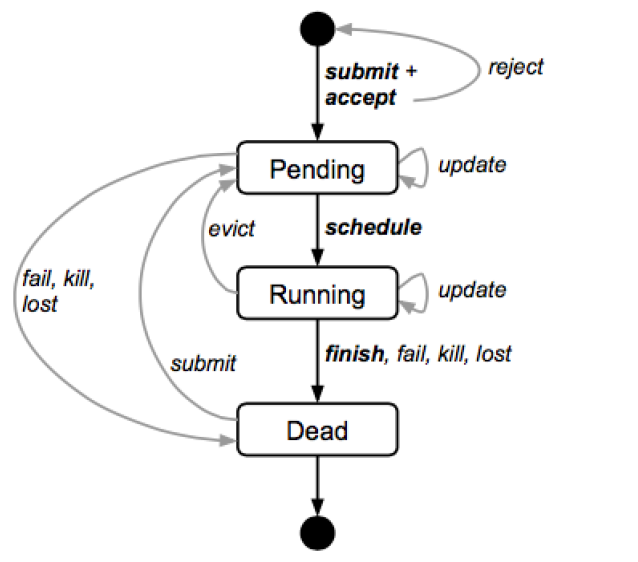
\includegraphics[width=0.5\linewidth]{images/borg_job_state_diagram.png}
			\caption{\textit{State diagram for both jobs and tasks. Users can trigger submit, kill, and update transitions.}}
		\end{figure}
		Users can interact with live jobs, this is achieved mainly using RPC. They can \textbf{update the specification of tasks}, while their parent job is running, updates are non-atomic and executed in a rolling-fashion.\newline
		Some task updates (e.g., pushing a new binary) will always require the task to be restarted; some (e.g., increasing resource requirements or changing constraints) might make the task no longer fit on the machine, and cause it to be stopped and rescheduled; and some (e.g., changing priority) can always be done without restarting or moving the task.
		\subsubsection{Allocs}
		A Borg alloc (short for allocation) is a \textbf{reserved set of resources on a machine} in which one or more tasks can be run; \textbf{the resources remain assigned whether or not they are
		used}.\newline
		Allocs can be used to set resources aside for future	tasks, to retain resources between stopping a task and starting it again, and to gather tasks from different jobs onto the	same machine.\newline
		An alloc \textit{set} is like a job: it is a group of allocs that reserve resources on multiple machines. \textbf{Once an alloc set has been created, one or more jobs can be submitted to run in it}.
		\subsubsection{Priority, Quota and Admission control}
		These are mechanisms to deal with resource demand and offer when more work shows up than can be accommodated (this is not scheduling, it is more admission control).\newline
		Job priorities are divided in non-overlapping bands for different uses, tasks from high-priority jobs can preempt low-priority tasks. Cascade preemption is avoided by disabling it for same-band jobs.\newline
		\newline
		Job/User quotas are used to decide which job to admit for scheduling. They are expressed as a vector of resource quantities at a given priority, for a period of time.\newline
		Pricing is the underlying mechanism to regulate user behaviour, it aligns user incentives to better resource utilization and discourages over-buying by over-selling quotas at lower priority.
		\subsubsection{Naming services}
		The Borg Name Service (BNS) is a mechanism to assign a name to tasks starting from cell name, job name and task number.\newline
		It uses the Chubby coordination service, it writes task names, health information and status. It is used by Borg RPC mechanism to establish communication	endpoints.\newline
		The DNS service inherits from BNS.
		\subsubsection{Monitoring services}
		Almost every task in Borg has a built-in HTTP server that provides health information and performance metrics.\newline
		The SIGMA service provides a monitoring UI with state of jobs, cells and tasks.\newline
		If a job is not running	Borg provides a “why pending?” annotation, together with guidance on how to modify the job’s resource requests to better fit the cell ("debugging service").\newline
		Billing services use monitoring information to compute usage-based charging, they help users debug their jobs and are used for capacity planning.
	\subsection{Architecture}
		\subsubsection{Borg master}
		The Borgmaster is one per Borg Cell, it orchestrates cell resources. It is composed of the \textbf{Borgmaster process} and the \textbf{scheduler process}.\newline
		The Borgmaster process handles client RPCs that either mutate state or lookup for state. It manages the state machines for all Borg “objects” (machines, tasks, allocs...), communicates with all Borglets in the cell and provides a Web-based UI.\newline
		\newline
		Borgmaster \textbf{reliability is achieved through replication}: the single logical process is replicated 5 times in a cell. The \textbf{master is elected using Paxos} when starting a cell, or upon failure of the current master. The Master serves as Paxos leader and cell state mutator.\newline
		Borgmaster replicas maintain an \textbf{in-memory} fresh copy of the cell state, they persist their state to a distributed Paxos-based store and help building the most up-to-date cell state when a new master is elected.\newline
		\newline
		Borgmaster \textbf{checkpoints its state} (time-based and event-based mechanism). The state includes everything related to a cell.\newline
		Checkpoints are used to restore the state to a functional one, e.g. before a failure or a bug, study a faulty state and fix it by hand, build a persistent log of events for future queries or for offline simulations.\newline
		\newline
		The \textbf{fauxmaster} is a high-fidelity simulator, it reads checkpoint files, accepts RPCs to make state machine changes and connects to simulated Borglets that replay real interactions from checkpoint files.\newline
		It helps users debug their application, make capacity planning, e.g. “How many new jobs of this type would fit in the cell?” and perform sanity checks for cell configurations, e.g. “Will this new configuration evict any important jobs?”.
		\subsubsection{Scheduling}
		New submitted jobs are stored in the Paxos store (for reliability) and put in the \textit{pending queue}. The scheduler process \textbf{operates at the task level}, it scans asynchronously the pending queue and assigns tasks to machines satisfying constraints.\newline
		The scanning is based on priority, within the same class, scheduling uses a round robin mechanism to ensure fairness and avoid blocking.\newline
		\newline
		The scheduling algorithm has two main processes. The \textbf{feasibility checking} finds a set of machines that meet the task's constraints (including resources already assigned to lower priority tasks).\newline
		The \textbf{scoring} process ranks machines from the previous one in order to minimize the number and priority of preempted tasks, prefer machines with a local copy of task's binaries and dependencies, spread tasks across failure and power domains, and mix high and low priority tasks on the same machine (to allow the former ones to expand).\newline
		\newline
		The scoring mechanism used to work with \textbf{worst-fit scoring}: it minimized the change in cost when placing a new task, this approach its good to spread tasks, it leaves headroom for load spikes but leads to fragmentation.\newline
		A better approach is the \textbf{best-fit scoring} which leaves empty machines that can be used for large tasks but, on the other hand, makes it difficult to deal with load spikes as the headroom in each machine highly depends on load estimation.\newline
		The solution used in practice is an hybrid which tries to reduce the amount of stranded resources.\newline
		\newline
		One of the most important metrics to optimize is the \textbf{startup latency} (time from job submission to running task), it deeply \textbf{depends on binaries and package installation}, therefore a possible solution is to place tasks on machines that already have dependencies installed.
		\subsubsection{Borglet}
		The Borglet is a Borg agent present on every machine in a cell.\newline
		It starts and stops tasks, and restarts failed tasks.\newline
		It manages machine resources interacting with the OS.\newline
		It maintains and rolls over debug logs.\newline
		It reports the state of the machine to the Borg master.\newline
		\newline
		Interaction with the Borg master uses a pull-based mechanism (heartbeat like), the Borglet continues operating even if the communications are interrupted. A failed Borgled is blacklisted and all its tasks are rescheduled.\newline
		The Borg master as to perform \textbf{flow and rate control} to avoid message flooding and many borgmaster replicas receive state updates. In order to handle the message overhead, the \textbf{link shard mechanism} is used: each replica communicates with a subset of the cell (partitioning is computed at each leader election), and the link shard mechanism aggregate state information. Differential state update is used to reduce the load of the master.
		\subsubsection{Scalability}
		Scalability is achieved through the decentralized design: the scheduler process is separated from the Borg master process and there is one scheduler per Borg master replica. Scheduling is somehow decentralized and states changes are communicated from replicas to the elected Borg master that finalized the state update.\newline
		Additional techniques are used to improve scalability: score caching, equivalence class and relaxed randomization.
	\subsection{Behaviour}
		\subsubsection{Availability}
		In large scale systems, failure are the norm. The baseline techniques to achieve high availability are replication, checkpointing and storing persistent state in a distributed file system.\newline
		Some additional techniques are: automatic rescheduling of failed tasks, mitigating correlated failures, rate limitation, avoid duplicate computation, admission control to avoid overload and minimization of external dependencies for task binaries.
		\subsubsection{System Utilization}
		To measure system utilization a sophisticated metric is used: \textbf{Cell Compaction}. The fauxmaster is used to compute it: given a workload in a point in time, remove physical machines at each iteration and exit the loop when the workload can no longer fill the cell size.\newline
		\newline
		\textbf{Cell sharing} has its benefits: Borg can reclaim resources unused by production jobs.\newline
		\textbf{Large cells} can accommodate large jobs and avoid fragmentation too.\newline
		Borg users specify job's requirement in terms of \textbf{fine-grained resource requests}, fixed size containers would require more machines in a cell.\newline
		Borg uses a \textbf{resource reclamation} system and it builds estimates of resource usage called \textbf{resource reservations}. Production jobs only rely on resources limits.
		\subsubsection{Isolation}
		Many tasks may interfere with each other, to obtain performance isolation borglets operate on the OS to control Linux containers resources, assigning resources based on predicted future usage or memory pressure.\newline
		Additional techniques are: application classes (latency sensitive or batch), resource classes (compressible or non-compressible) and OS tuning, especially the OS scheduler.
	\subsection{Lesson Learned}
		\subsubsection{The bad}
		The job abstraction is to simplistic, multi-job services cannot be easily managed or addressed.\newline
		The addressing service is critical, one IP address implies managing ports as a resource, which complicates tasks.\newline
		Borg is more geared to power users than casual ones.
		\subsubsection{The good}
		Allocs are a useful resource envelope for one or more containers sharing resources and co-scheduled on the same machine.\newline
		Cluster management is more than task management.\newline
		Introspection is vital for debugging, capacity planning and monitoring.\newline
		The cooperation of micro-services that use a common low-level API to process requests and manipulate state is good.
	